\documentclass[14pt,fleqn]{extarticle}
\RequirePackage{prepwell}
\previewoff
\begin{document}

%text
Find the equation of the tangent to the 
curve $y = \sqrt{3x - 2}$ which is parallel to the 
line $4x-2y +5 =0$.
%

\newcard 

\begin{center}
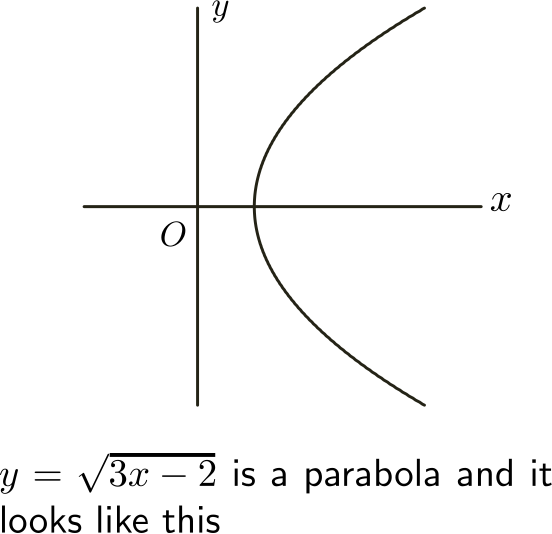
\includegraphics[scale=0.4]{r-1.svg} 
\end{center} 

\newcard 

\begin{center}

\includegraphics[scale=0.4]{w-1.svg}
\end{center} 

\newcard 

$y= \sqrt{3x-2}$ is defined only when 
\[ \qquad 3x - 2 \geq 0 \implies x \geq \frac{2}{3}\]

Which means that there can be 

\underline{no curve for $x < \frac{2}{3}$} \newline 

Moreover $y = \sqrt{3x-2} \implies y^2 = \left(3x-2 \right)$ \newline 

And that is the equation of a parabola that opens to the right (towards positive x-axis) 

\begin{center}
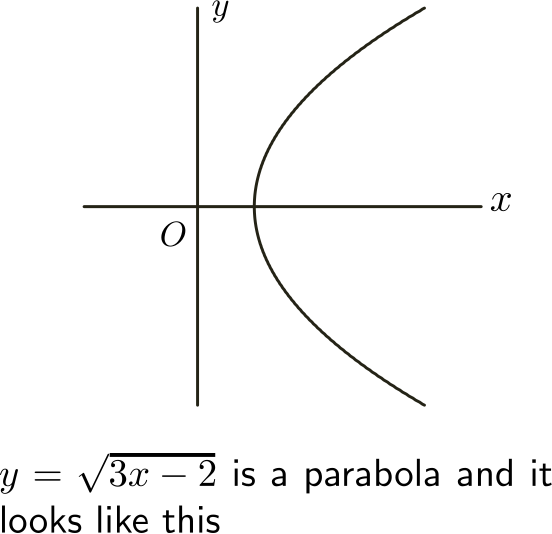
\includegraphics[scale=0.25]{r-1.svg} 
\end{center} 

\newcard 

For the required tangent to be parallel to $4x-2y+5=0$, 
\[ \quad \qquad \frac{3}{2\sqrt{3x-2}} = 2 \]

\newcard 

For the required tangent to be parallel to $4x-2y+5=0$, 
\[ \quad \qquad \frac{3}{\sqrt{3x-2}} = 1 \]


\newcard 

The slope of the tangent is simply 
\[\frac{d}{dx}\sqrt{3x- 2} = \frac{1}{2\sqrt{3x-2}}\cdot 3 = \frac{3}{2\sqrt{3x-2}} \]

Moreover, the slope of the given line is 
\[ 4x-2y + 5 = 0 \implies y = 2x + \frac{5}{2} \implies m = 2 \]

And therefore, for the tangent to be parallel to the given line
\[ \qquad \frac{3}{2\sqrt{3x-2}} = 2 \]

\newcard 

\begin{align}
	\frac{3}{2\sqrt{3x-2}} &= 2 \implies 3x - 2 = \left(\frac{3}{4} \right)^2  \\
	\implies x &= \frac{41}{48} \text{ and } y = \sqrt{3x-2} = \pm \frac{3}{4} 
\end{align}

But only the tangent at  
\[ \qquad A = \left(\frac{41}{48}, \frac{3}{4} \right)\]
can be parallel to the given line 

\newcard 

\begin{align}
	\frac{3}{2\sqrt{3x-2}} &= 2 \implies 3x - 2 = \left(\frac{3}{4} \right)^2  \\
	\implies x &= \frac{41}{48} \text{ and } y = \sqrt{3x-2} = \pm \frac{3}{4} 
\end{align}

Which means there are two points 
\[ A = \left(\frac{41}{48}, \frac{3}{4} \right) \text{ and } B = \left(\frac{41}{48}, -\frac{3}{4} \right)\]

at which the tangent is parallel to the given line 

\newcard 

\begin{center}
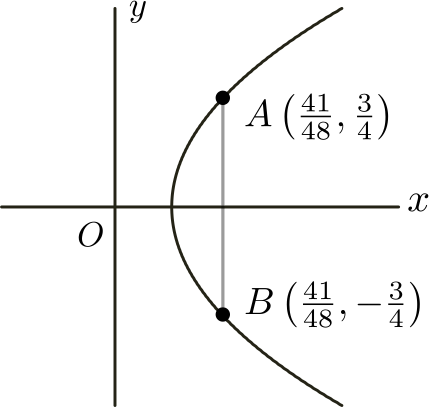
\includegraphics[scale=0.3]{rs-2.svg} 
\end{center} 

$\dfrac{3}{2\sqrt{3x-2}} = 2 \implies x = \frac{41}{48}$ \newline 

However, \underline{for the same $x$} we have two points $A$ and $B$ on the parabola \newline 

And one can see that only the tangent at $A$ will have slope $m > 0$ -- which is what we need \newline 

The tangent at $B$, on the other hand, will be downward sloping -- which means - $m < 0$ \newline 

Hence, $A$ is the only acceptable point


\newcard

The required tangent (at point $A$) is 
\[ \qquad 24y = 48x - 23 \] 


\newcard

%text
As the required tangent passes through 

$A = \left(\frac{41}{48},\frac{3}{4} \right)$ and has slope $m = 2$, therefore

\begin{align}
\dfrac{y-\frac{3}{4}}{x-\frac{41}{48}} = 2 &\implies y-\frac{3}{4} = 2x-\frac{41}{24} \\
\text{or } 24y &= 48x - 23 
\end{align}

\end{document}
